\section{问题二：无日内调账的因果分位轨迹优化}

\subsection{滚动相似日预测}

问题二要求在每天开始前一次性确定全天合同，因而预测只能由过去日期生成。对目标日$d$，取最近90日内的历史日期集合 $\mathcal H_d$。对负荷，目标日与历史日星期属性相同时附加权重2，否则权重1；光伏不使用星期加权。时间衰减统一为
\begin{equation}
 \omega_{dk}=a_{dk}\exp\!\left(-\frac{d-k}{60}\right),\qquad k\in\mathcal H_d,
 \label{eq:analogweight}
\end{equation}
其中 $a_{dk}=2$ 或1。历史样本较少时，将加权历史均值向附件典型日收缩。以负荷为例，
\begin{equation}
 \widehat L_{d,t}=\gamma_d
 \frac{\sum_{k\in\mathcal H_d}\omega_{dk}L_{k,t}}
 {\sum_{k\in\mathcal H_d}\omega_{dk}}
 +(1-\gamma_d)L_t^{\mathrm{typ}},
 \qquad \gamma_d=\min\left(1,\frac{|\mathcal H_d|}{21}\right).
 \label{eq:analog}
\end{equation}
首日没有历史时直接采用典型日；光伏采用相同结构但 $a_{dk}=1$。该收缩使冷启动平滑过渡到滚动历史估计，不需要把未来全年样本先用于训练。

图\ref{fig:q2-raw}展示365日净负荷 $P_{\mathrm{load}}-P_{\mathrm{pv}}$ 的季节和日内结构。正负区间交替说明光伏富余与负荷缺口都具有显著时变性；仅用单个年度均值无法形成可执行合同。

\begin{figure}[H]
  \centering
  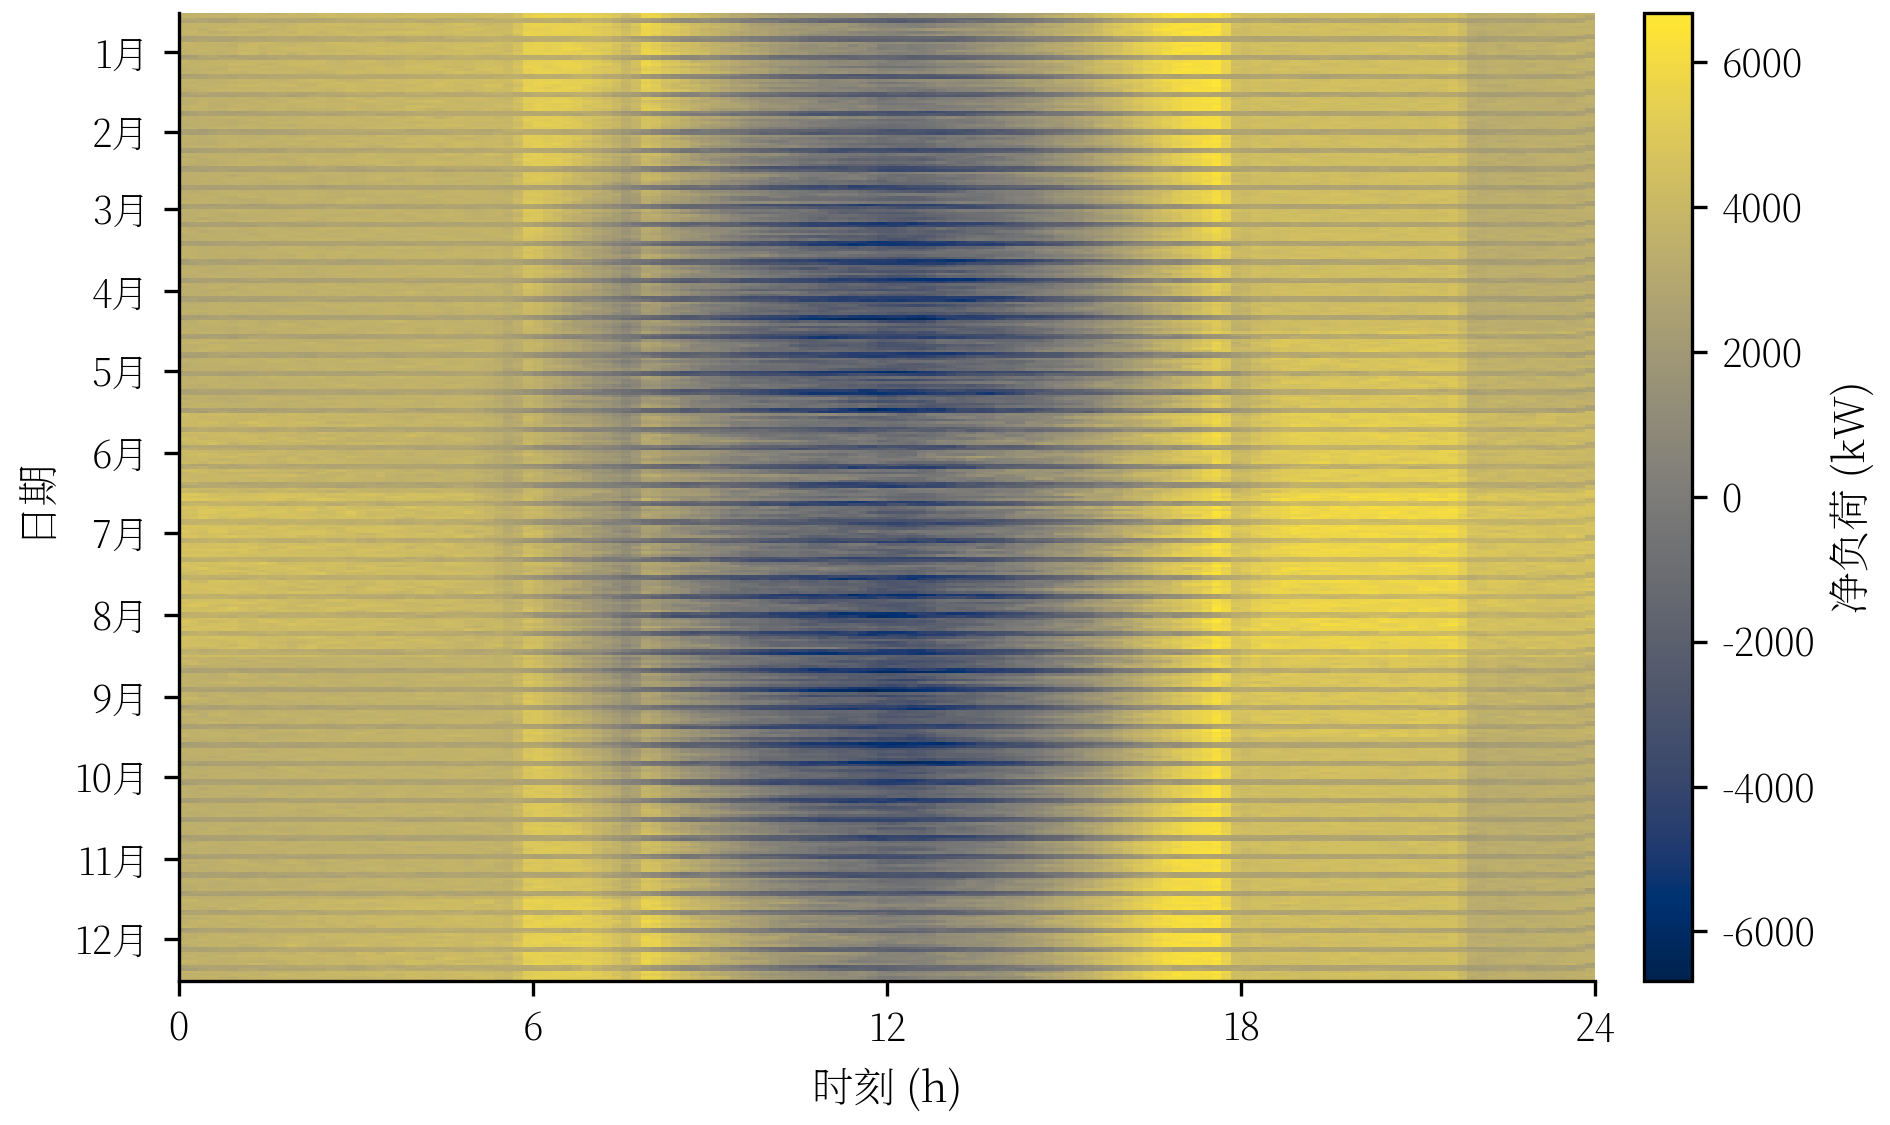
\includegraphics[width=0.98\textwidth]{figs/raw_q2_annual_netload.png}
  \caption{2025年365日净负荷的季节--日内分布。该图使用全年原始数据，策略费用统计期另为2月至12月。}
  \label{fig:q2-raw}
\end{figure}

在正式统计期上，相似日负荷预测 MAE 为 $722.5708\,\mathrm{kW}$，RMSE 为 $904.0899\,\mathrm{kW}$；光伏预测 MAE 为 $335.9217\,\mathrm{kW}$。图\ref{fig:q2-forecast}表明多数点接近45度线，但仍存在明显尾部误差。因此，单纯把点预测当作确定真值会低估应急购电风险。

\begin{figure}[H]
  \centering
  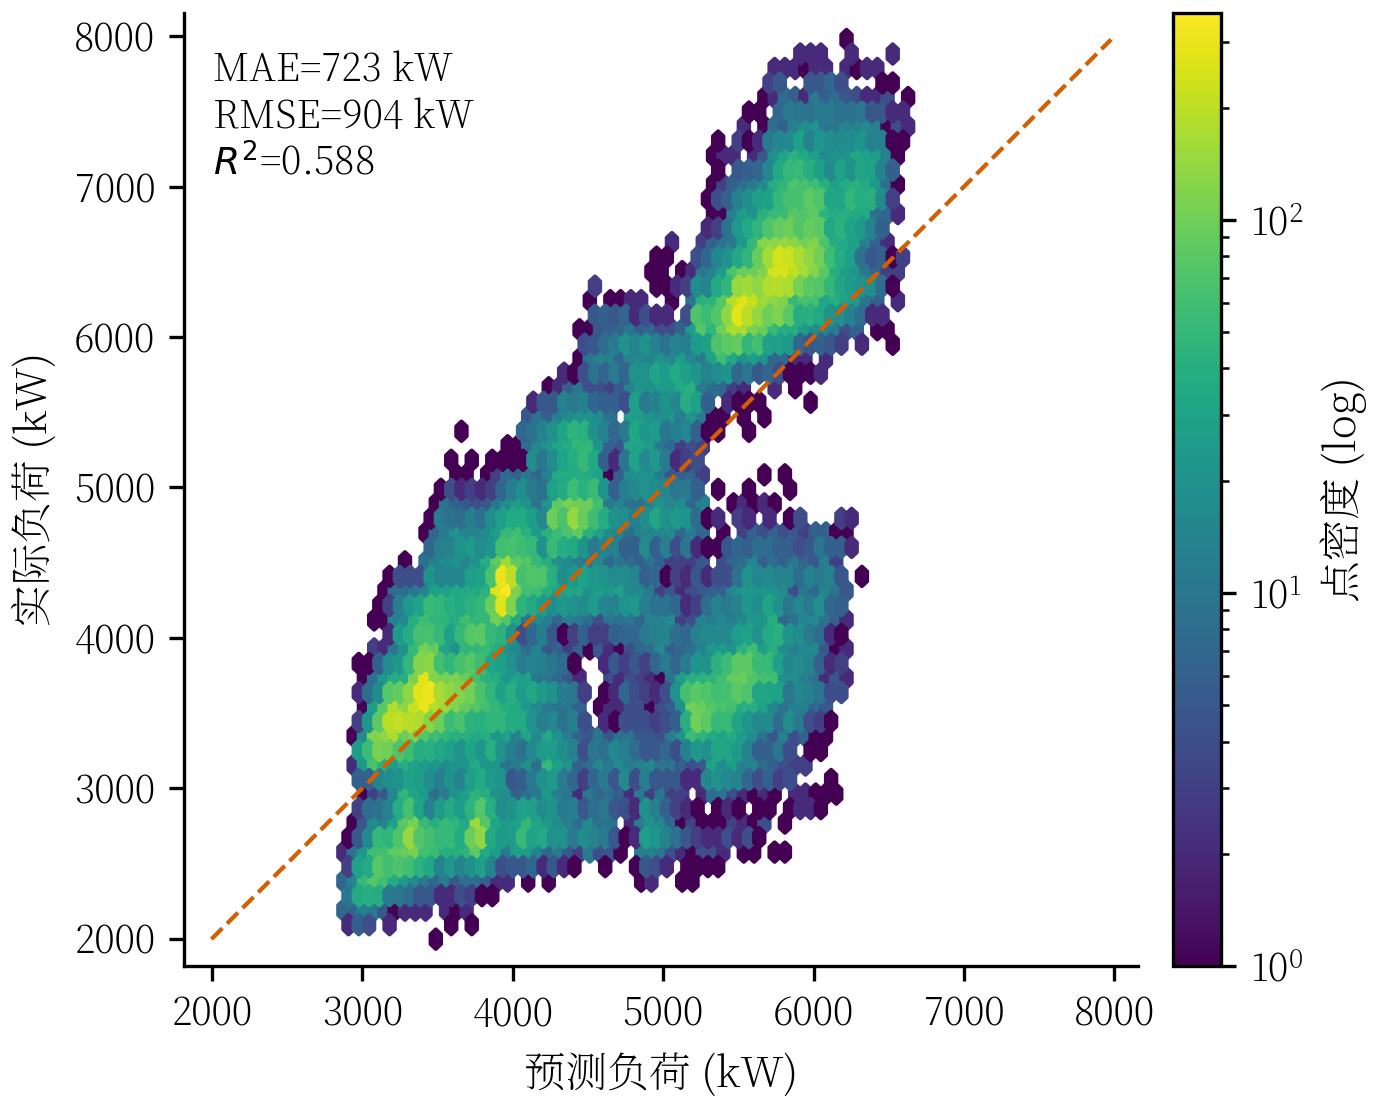
\includegraphics[width=0.72\textwidth]{figs/process_q2_forecast_validation.png}
  \caption{2月至12月因果相似日负荷预测与真实负荷的比较。颜色表示样本密度，离45度线较远的点对应尾部误差。}
  \label{fig:q2-forecast}
\end{figure}

\subsection{联合残差场景与边际分位压缩}

定义负荷和光伏残差
\begin{equation}
 e^{L}_{d,t}=L_{d,t}-\widehat L_{d,t},\qquad
 e^{V}_{d,t}=V_{d,t}-\widehat V_{d,t}.
 \label{eq:residual}
\end{equation}
在日期$d$只取最近60个已完成日期的残差，将一天的两类残差拼接为288维向量，并按各维历史标准差标准化。标准差小于 $10^{-9}$ 时置为1，避免近常数维放大数值误差。随后用 $K$-means 将残差日聚为至多9类，随机种子固定为2026，重复初始化10次；实际簇数不超过历史样本中唯一残差向量数。空历史退化为一个零残差场景，单条历史保留该样本本身。

设第$s$个场景的负荷和光伏轨迹为 $L^{(s)}_t,V^{(s)}_t$，簇权重为 $\pi_s$。对净负荷 $N^{(s)}_t=L^{(s)}_t-V^{(s)}_t$ 取加权经验 $\alpha$ 分位数，对光伏取 $1-\alpha$ 分位数：
\begin{align}
 \widetilde N_t &= Q_{\alpha}\!\left(\{N^{(s)}_t,\pi_s\}\right),\\
 \widetilde V_t &= \max\left\{Q_{1-\alpha}\!\left(\{V^{(s)}_t,\pi_s\}\right),-\widetilde N_t,0\right\},\\
 \widetilde L_t &= \widetilde V_t+\widetilde N_t.
 \label{eq:safe-trajectory}
\end{align}
经验分位数采用累计权重首次达到阈值的样本，不作线性插值。主方案在计算前固定 $\alpha=0.8$。式\eqref{eq:safe-trajectory}分别保守化净负荷和光伏，并通过重构保证 $\widetilde L_t,\widetilde V_t\ge0$ 及二者净差一致。

这种压缩保留了“净需求偏高、可用光伏偏低”的风险方向，却不再保留完整的跨时段联合分布。因此，后续优化应称为边际分位轨迹线性规划，而不是完整随机MPC。滚动残差给出的名义90\%经验区间对负荷、光伏的实际覆盖率分别为83.1109\%和83.4581\%，均低于90\%；它只能作为历史回测描述，不能构成概率保证。

从实现顺序看，每个日期的预测与规划包含五个确定步骤。首先读取不超过当前日期的历史索引，并生成相似日点预测；其次在历史残差上进行退化检查和标准化；再次聚类得到代表残差与经验权重；随后按式\eqref{eq:safe-trajectory}逐槽取分位数并重构安全负荷；最后以当天实际SOC为初态求解144槽LP。当天结束后才把真实残差加入下一日历史。该顺序保证“先预测、后观察、再更新历史”，不会因为一次性载入全年附件就把未来行用于当前决策。

选择边际分位压缩而没有直接对所有场景逐一设置供电约束，主要基于两点。其一，题目要求连续运行334个正式日期并完成54组实验，压缩后每次规划规模固定，便于稳定求解和逐槽复核；其二，分位参数 $\alpha$ 直接对应净负荷上侧与光伏下侧的保守方向，能够通过敏感性曲线解释风险偏好。代价是场景之间的时序相关只用于形成代表样本，进入LP后被一条轨迹替代。因此，本文把场景聚类视为风险特征提取，而非声称求解了多阶段随机规划。

\subsection{日前合同优化与真实执行}

在日期$d$的0时，用安全轨迹 $(\widetilde L_t,\widetilde V_t)$ 代替未知真实轨迹，求解统一物理模型。固定电价下，规划目标写为
\begin{equation}
 \min\ \sum_{t=0}^{143}c_tg_t-\lambda_d S_{144},
 \qquad \lambda_d=\eta_d\operatorname{median}\{c_t:t\text{属于剩余规划域}\}.
 \label{eq:q2plan}
\end{equation}
末端价值 $\lambda_d S_{144}$ 防止算法在一天末尾无代价地放空电池，但报告现金费用时不扣除这项信用。优化完成后合同 $g_t$ 全天不再改变。

真实槽到达时，执行层只使用当前真实负荷和光伏。若光伏及合同供给有余量，则先在功率和SOC允许范围内充电，之后的合同剩余计为闲置合同，光伏剩余计为弃光；若有缺口，则先放电，仍不能满足的部分以5倍当前电价应急购电。这个优先级是透明的因果反馈规则，而不是用全天真实量重新优化。

规划层与执行层分离有一个重要含义：LP给出的充放电计划服务于安全轨迹，真实执行动作则必须服从已实现的供需和当前SOC。若真实光伏高于保守轨迹，额外余电优先充电；若真实负荷高于轨迹，电池可能比计划更早放电。因而“计划合同总量”与“实际购电供能量”不完全相同，现金费用也不能由计划目标值直接替代，必须逐槽按真实执行和应急量重新结算。

\subsection{年度结果与基线比较}

从2月1日至12月31日，无日内调账主策略现金费用为 $18764165.9334$ 元，其中普通合同结算为 $15258616.4937$ 元，应急费用为 $3505549.4397$ 元；应急购电量为 $578081.5436\,\mathrm{kWh}$，闲置合同电量为 $4123779.9049\,\mathrm{kWh}$，弃光为 $1950263.9848\,\mathrm{kWh}$。年末SOC为 $10609.7713\,\mathrm{kWh}$。每日费用和应急量具有明显异质性，见图\ref{fig:q2-risk}，图中的7日中心均线仅用于事后描述，不进入任何日前预测。

\begin{figure}[H]
  \centering
  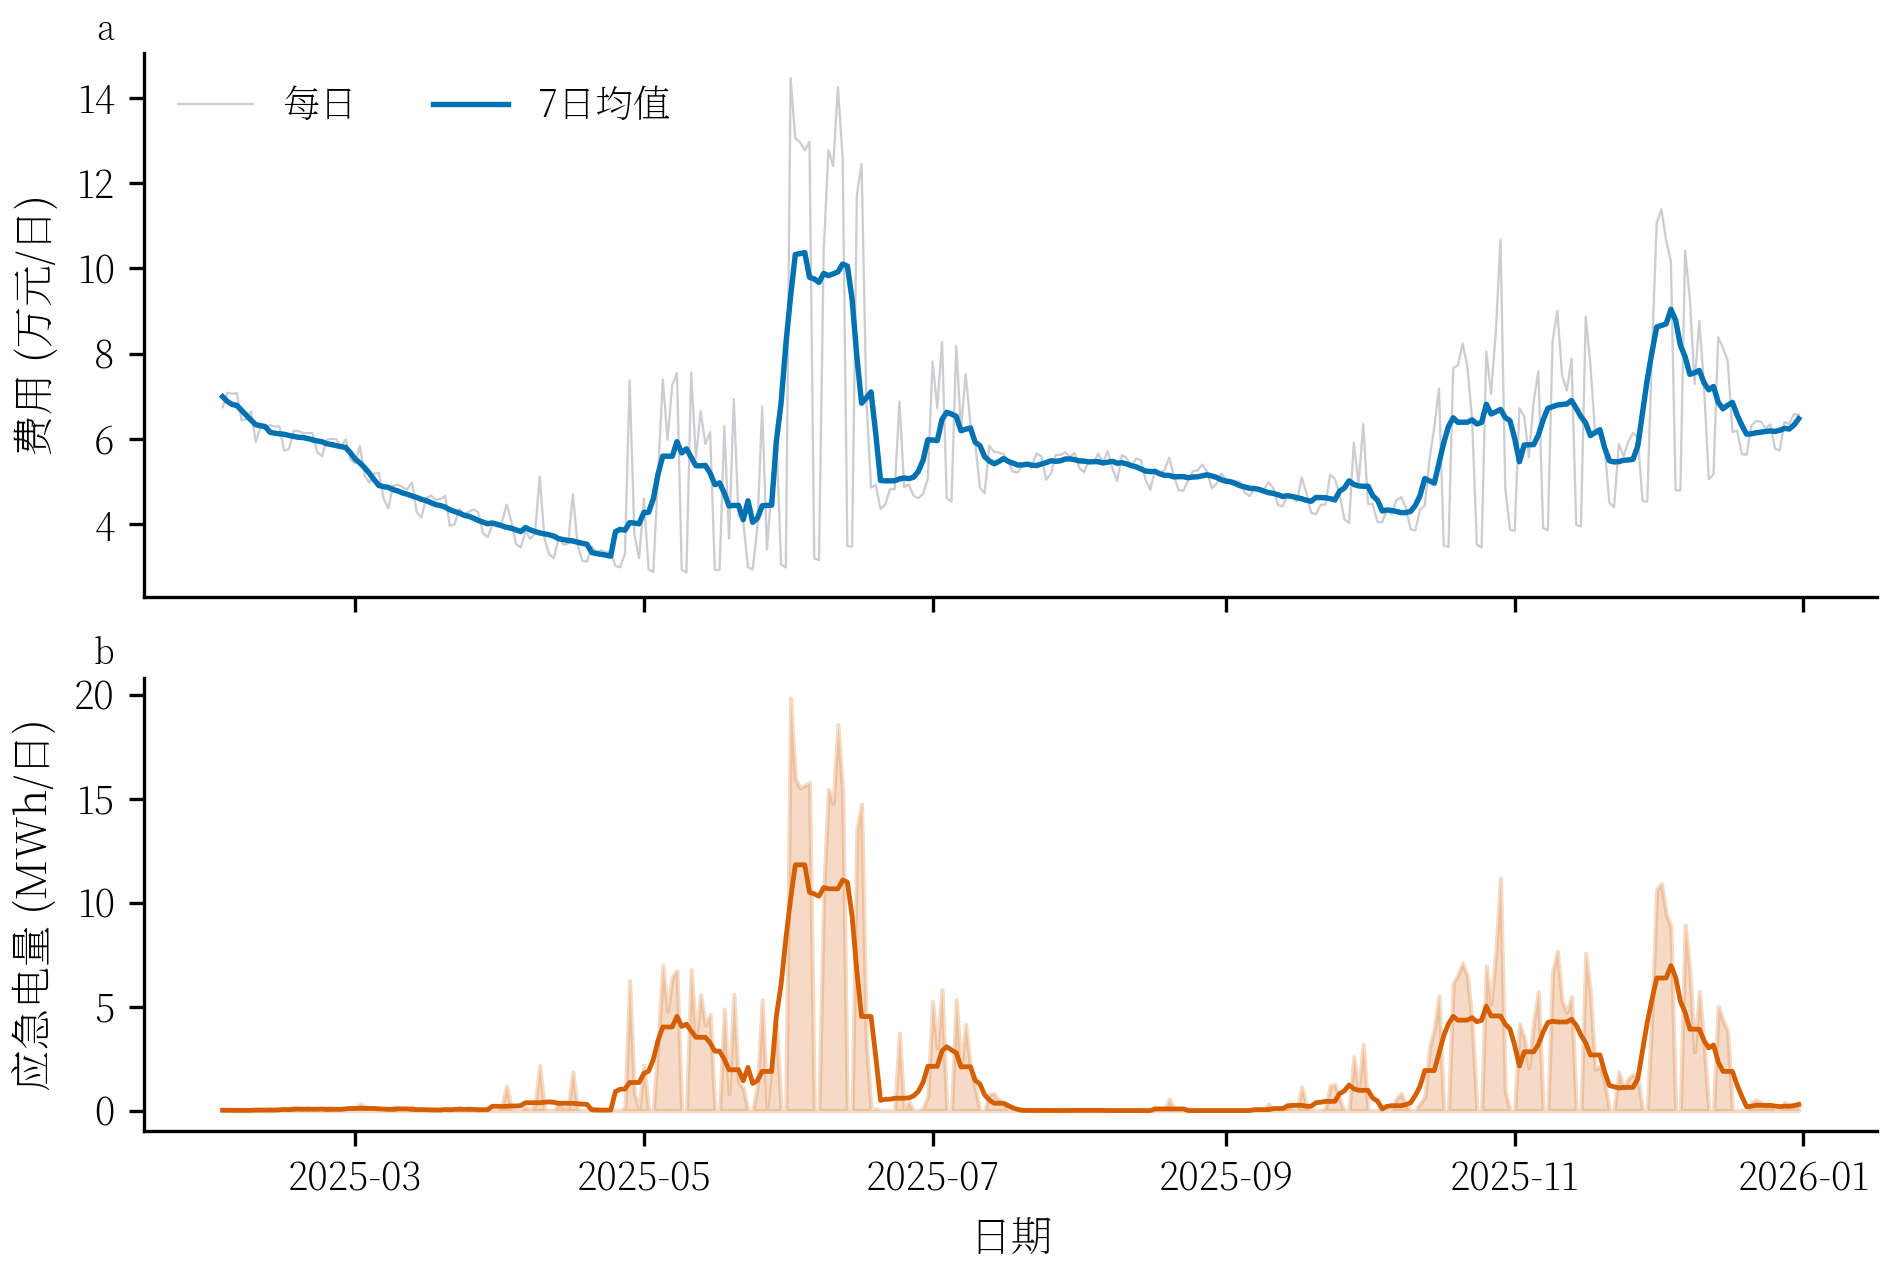
\includegraphics[width=0.98\textwidth]{figs/result_q2_annual_risk.png}
  \caption{问题二334日现金费用与应急购电量。原始日值显示尾部风险，中心均线不作为模型输入。}
  \label{fig:q2-risk}
\end{figure}

为判断保守轨迹的作用，比较点预测、典型日和无储能三类基线。表\ref{tab:q2base}显示，点预测和典型日方案都因应急购电显著增加而费用较高。无储能方案费用低于这两项，却仍高于保守轨迹主策略；它的应急量与主策略相近，但弃光更高，说明储能和合同保守度必须联合考察，不能只看应急电量。

\begin{table}[H]
\centering
\caption{问题二主策略与基线的334日结果}
\label{tab:q2base}
\begin{tabular}{lrrr}
\toprule
策略 & 现金费用/元 & 应急购电/kWh & 弃光/kWh\\
\midrule
保守分位轨迹 & 18,764,165.93 & 578,081.54 & 1,950,263.98\\
点预测 & 27,574,292.97 & 2,685,630.97 & 1,618,696.22\\
典型日 & 27,753,076.30 & 2,724,419.83 & 1,773,185.71\\
无储能 & 21,799,176.46 & 609,913.86 & 3,058,159.92\\
\bottomrule
\end{tabular}
\end{table}

\noindent 图\ref{fig:q2-baselines}进一步把合同结算与应急费用分开。主策略普通合同部分较高，是对预测尾部风险的事前支付；点预测和典型日虽然减少合同购买，却把更多缺口暴露在5倍应急价格下。无储能方案没有充放损耗，但中午光伏难以跨时段转移，其弃光约305.82万kWh，显著高于有储能主策略。由此，主策略的优势不是单纯“买得更多”或“电池越大越好”，而是合同保守度与储能转移共同改变了高价缺口的位置和规模。

\begin{figure}[H]
  \centering
  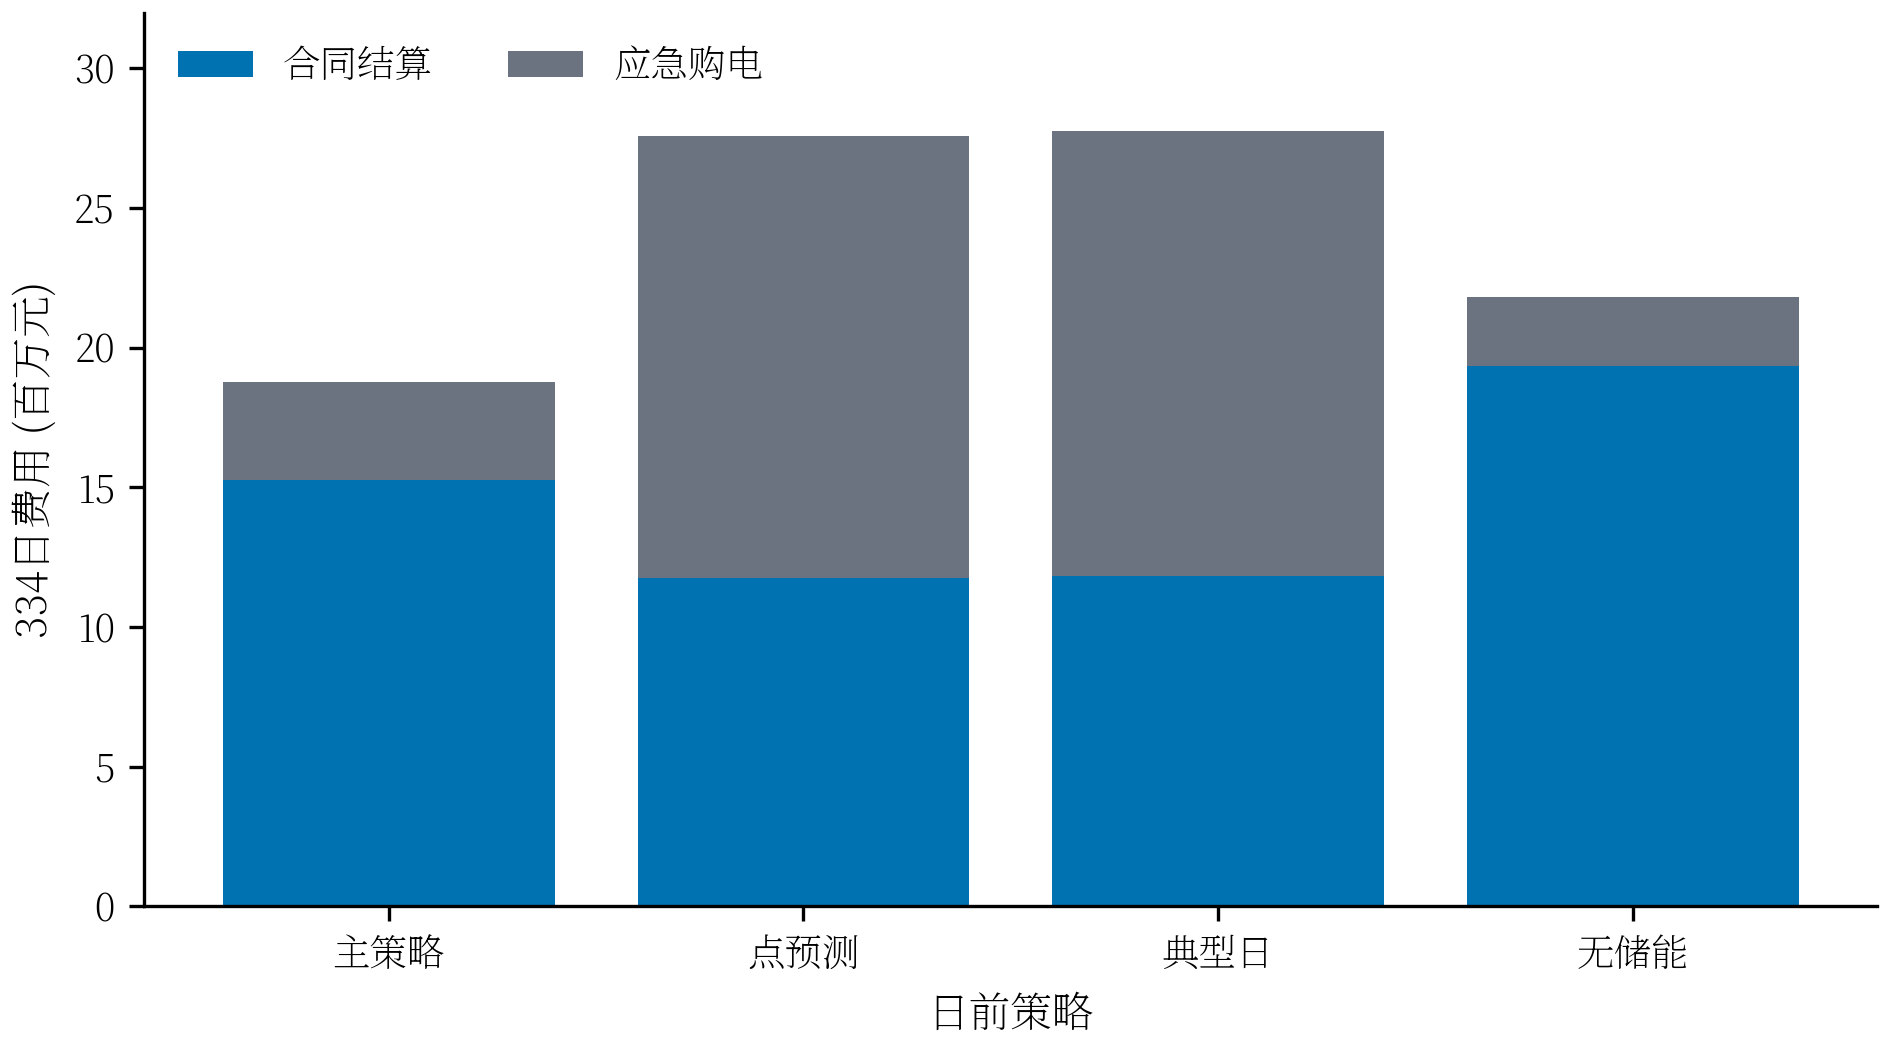
\includegraphics[width=0.96\textwidth]{figs/result_q2_baselines.png}
  \caption{问题二不同基线的合同费用与应急费用分解。柱高为334日总额，不表示抽样均值的置信区间。}
  \label{fig:q2-baselines}
\end{figure}

四个代表日的指定购电、储能和应急表分别列于附录\ref{app:tables}。代表日结果同时显示一个重要边界：策略在总体上降低风险，并不意味着每个日期都严格优于其他策略；这种日期异质性将在问题三中继续讨论。
